\chapter{Introduction}
\label{sec:Introduction}

\section{Motivation} %Wind Energy Conversion System Control} 
Wind energy plays a significant role in Germany's renewable energy landscape and provides a critical contribution to the national energy transition, with the share of electricity production from wind having increased from 8.4\% in 2013 to 27.2\% in~2023~\cite{EmberEI2024}. Wind turbines, also called Wind Energy Conversion Systems (WECS), help to meet a still increasing power demand sustainably. Unlike conventional energy sources, they neither emit greenhouse gases nor produce radioactive waste. A trend toward larger wind turbines maximizes energy yield per unit, thus enhancing the economic feasibility of wind power by lowering the Levelized Cost of Energy (LCoE). However, larger wind turbines necessitate efforts to minimize structural loads. This can be achieved both through optimized tower and blade designs~\cite{modelling2010006, Jasa_2022} as well as efficient control strategies~\cite{pao2011control}. %\cite{irena2023renewable}. 

Model Predictive Control (MPC) is a promising approach for managing aerodynamic and structural loads in wind turbines for several reasons, particularly due to its ability of making control decisions that account for future known or estimated events. This is highly beneficial for turbine control as wind conditions can vary rapidly. Another advantage of MPC is its capability to handle multiple control objectives. For wind turbines, these objectives include maximizing power output, minimizing mechanical loads to extend the turbine's lifespan, and maintaining system stability. MPC also excels in dealing with constraints on control actions and state variables, ensuring that all turbine operations remain within safe limits~\cite{Holm2013, pamososuryo2021loadcontrol}.

MPC is also well-suited for wind farm control as it can anticipate future wind conditions and turbine responses and is able to optimize the performance of multiple interconnected turbines while considering various operational constraints and objectives~\cite{boersma2017tutorial, meyers2022windfarmflow}. The predictive model of MPC allows the control system to make informed decisions about adjusting turbine settings before changes in wind speed and direction occur, maximizing energy production and reducing the risk of turbine wear due to abrupt changes in operating conditions in a farm~\cite{vali2017adjointbasedmodel}. In a wind farm, wakes can significantly reduce the wind speed downstream of a turbine and hence impact the performance of other turbines. MPC can control individual turbines in a coordinated manner to optimize the overall wind farm performance, taking into account the interactions between turbines due to wake effects~\cite{meyers2022windfarmflow}. Through coordinated control, MPC can manage the power output of each turbine to maximize the total energy production of the wind farm. It can intelligently reduce power output from certain turbines to mitigate wake effects on downstream turbines, thereby increasing the overall efficiency of the wind farm~\cite{vali2017adjointbasedmodel}.

In this work, physics-based MPC is applied for controlling individual turbines and data-driven MPC for wind farms. Individual turbines benefit from physics-based MPC because these models can capture the dynamics of turbine mechanics, aerodynamics, and their interactions with the wind. These models are based on first principles and well-understood physical laws, making them very accurate for predicting the performance and structural stresses on individual turbines.

Data-driven MPC is well-suited to model wake effects in wind farms. It can use large amounts of data, either directly or through data-driven models, to understand and predict the impact of these interactions better than purely theoretical models. The use of the Koopman Operator \cite{koopman1931hamiltonian} to build the model for a data-driven MPC offers an efficient, real-time-capable method for handling the complexities and dynamics of wind farms.

\subsection{Wind Turbine Control} 
Modern multi-megawatt wind turbines are both speed controlled and pitch control\-led~\cite{wright2008advanced}. The control of the wind turbine's rotor speed at low wind speeds aims at generating the maximum power amount possible by controlling the generator power either directly via the voltage or via the generator torque. Turbine control at high wind speed aims at lowering the Damage Equivalent Loads (DEL) acting on the structure by pitching the blades. Yaw control is used to turn WECSs into the wind. Further load alleviation can be done by controlling the blades individually or by adding additional control inputs, like Trailing Edge Flaps (TEF) \cite{zhang2015parameter}. This, however, requires that the corresponding hardware components are installed on the turbine, as TEFs are not standard equipment and must be mechanically integrated into the blade design. Load reduction was also shown to be achievable by including information from wind speed measurements from anemometers or Light Detection and Ranging (lidar) sensors into the control loop \cite{schlipf2013nonlinear}. Lidar information is particularly effective in MPC, where it is used to provide a preview of incoming wind conditions, allowing proactive adjustments that mitigate aerodynamic loads and improve efficiency.

The tower and blade modes targeted in controller design typically lie between 0.1\,Hz and 3\,Hz, a frequency range that includes their first and second modes. While higher-frequency dynamics, such as torsional modes of the drivetrain occurring in the 4\,Hz to 6\,Hz range, can be relevant for detailed modeling, they tend to be neglected in WECS control design, which is focused on the most relevant low-frequency turbine modes. Some wind fluctuations can occur below 0.1\,Hz. A commonly used benchmark for modern utility-scale wind turbines is the NREL 5MW reference turbine, developed to represent typical dynamic and structural properties of multi-megawatt turbines~\cite{jonkman2009definition}. This turbine model is also used for all simulations presented in this thesis. For the NREL 5MW, the first tower fore-aft and blade flapwise modes occur at approximately 0.3\,Hz and 0.7\,Hz, respectively, with second blade modes and the second tower mode occurring between 1.9\,Hz and 2.9\,Hz. Collective Pitch Control (CPC) and generator torque control primarily address dynamics in the 0.01\,Hz to 0.7\,Hz range, with pitch focusing on power regulation as well as gust and load mitigation, and torque control optimizing power capture and damping drivetrain oscillations. Controllers typically update around 10\,ms (100\,Hz), allowing real-time management of faster wind fluctuations, structural dynamics, and loads. Yaw control operates considerably more slowly to align the rotor with the wind. The yaw controller of the NREL 5MW is updated at 3\,Hz and has a rate limit of 0.3\textdegree/s. There are different strategies: yaw might be actuated only if the accumulated, low-pass filtered yaw error exceeds a certain threshold within a given time to minimize yaw motor wear, e.g., 10\textdegree{} in ten minutes~\cite{fleming2014yawmisalignment}. Modern yaw controllers can have a continuous, real-time update to maintain alignment with the wind~\cite{stanley2022yawoptimization}, which potentially slightly increases yaw actuator wear, but increases power output and decreases DELs due to misalignment.
 
An exploration of Active Aerodynamic Load Control (AALC) technologies that adjust rotor blade control inputs together with add-ons like TEFs has demonstrated significant potential to decrease fatigue and structural wear and thereby extending the lifespan of wind turbines. Detailed investigations into Individual Pitch Control (IPC) and TEF control as methods to actively manage aerodynamic loads are a promising approach for reducing blade root and tower base bending moments. AALC aims to address structural challenges and enhance the efficiency and durability of wind turbines, see~\cite{aubrun2017review} for a survey on AALC.

In this work, different control strategies are compared: MPC with CPC, IPC with a classical Proportional-Integral (PI) controller, and IPC combined with TEFs. The quantitative comparison criterion is their effectiveness in DEL reduction. The evaluation highlights the potential of MPC, particularly in its ability to minimize fatigue on key structural components such as the blade root and tower base. In addition, evaluating these methods under similar operating conditions, the potential synergies of IPC and TEF control are also explored to assess their combined impact on overall load alleviation and power production.

This work utilizes the software Fatigue, Aerodynamics, Structures, and Turbulence (FAST) \cite{jonkman2005fast}, a mid-fidelity wind turbine simulation tool developed by the National Renewable Energy Laboratory (NREL). FAST models the dynamic behavior of wind turbines, capturing aeroelastic interactions and control system responses. For baseline control, the MATLAB/Simulink-based FASTTool~\cite{mulders2020wind} from Delft University of Technology (TU Delft) is used, which integrates FAST as an S-Function for modeling the wind turbine.


\subsection{Wind Farm Control}
Modern wind farms are designed to optimize power generation across multiple turbines while minimizing overall structural loads and extending the lifespan of the equipment. The current state-of-the-art in wind farm control primarily involves farm-level controllers that distribute power references to individual turbines. These farm controllers keep the farm power output as close as possible to a power grid reference, while individual turbines execute these references using their own local control systems. 

Advanced control strategies such as Axial Induction Control (AIC) and Wake Redirection Control (WRC) have demonstrated significant potential to increase wind farm power yield and to lower mechanical loads in simulations and field tests~\cite{houck2022review}. AIC modifies the axial induction factor of individual turbines to influence wake structures. The axial induction is the difference in wind speed of the freestream wind speed and the wind speed at the turbine's rotor. It can be changed by influencing the thrust via the generator torque or the blade pitch. WRC adjusts turbine yaw angles to deflect wakes away from downstream turbines, reducing interference and enhancing overall energy capture. However, these techniques are not yet widely adopted in practice due to challenges in integrating them into existing control systems and uncertainties in wake modeling \cite{andersson2021wind, houck2022review}.

The development and testing of these advanced strategies are supported by sophisticated wind farm software tools, which simulate turbine interactions and optimize performance based on wake dynamics, turbine loads, and power production goals. As computational models and field validations continue to advance, these emerging strategies hold promise for inclusion in next-generation wind farm control systems, offering the potential to further enhance energy yields and operational reliability \cite{stock2024wind}.

The simulation tool WFSim (Wind Farm Simulator) \cite{boersma2018control} from TU Delft was used in this work for wind farm simulation. WFSim employs a linearized version of the Navier-Stokes Equations (NSE) to model wake dynamics, capturing key behaviors such as momentum transport and diffusion while ensuring short simulation times. Turbines are implemented as actuator disk models, representing rotor aerodynamic effects by imposing momentum deficits and turbulence generation within the flow field.

\section{Related Work}
Both wind turbine and farm control are very active areas of research. Several other research groups achieved results slightly prior to the start of this PhD project or while it was ongoing. Figures~\ref{fig01:WTstatistics} and~\ref{fig01:WFstatistics} show the results of automated Google Scholar searches for different search terms to visualize the historical activity per year of research subjects discussed in this thesis. The search terms and scripts used to generate these results are available for reproducibility in \cite{dittmer_scholar}. These results are not intended as a comprehensive  analysis, but rather as a simple illustrative overview of publication trends in the field.
% 16 MPC for 2010

\begin{figure} [h]
 \center
 \subfloat[Search terms ``load reduction'' and ``individual pitch control"]{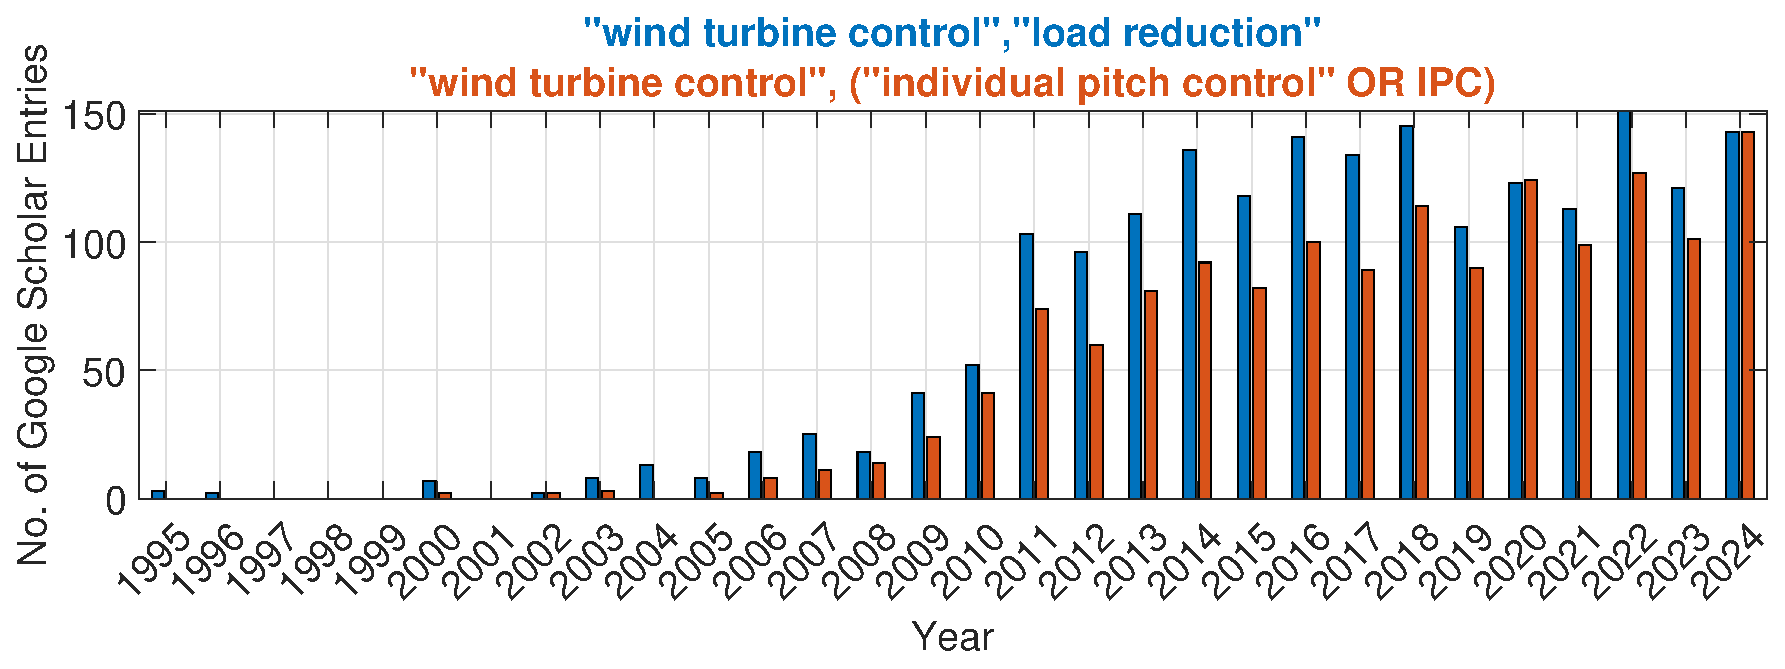
\includegraphics[width=0.85\textwidth]{figures/Figures_ADi/googleWordleWTLoadRedIPC.eps}} \\ %\hfill 
 \subfloat[Search term ``model predictive control"]{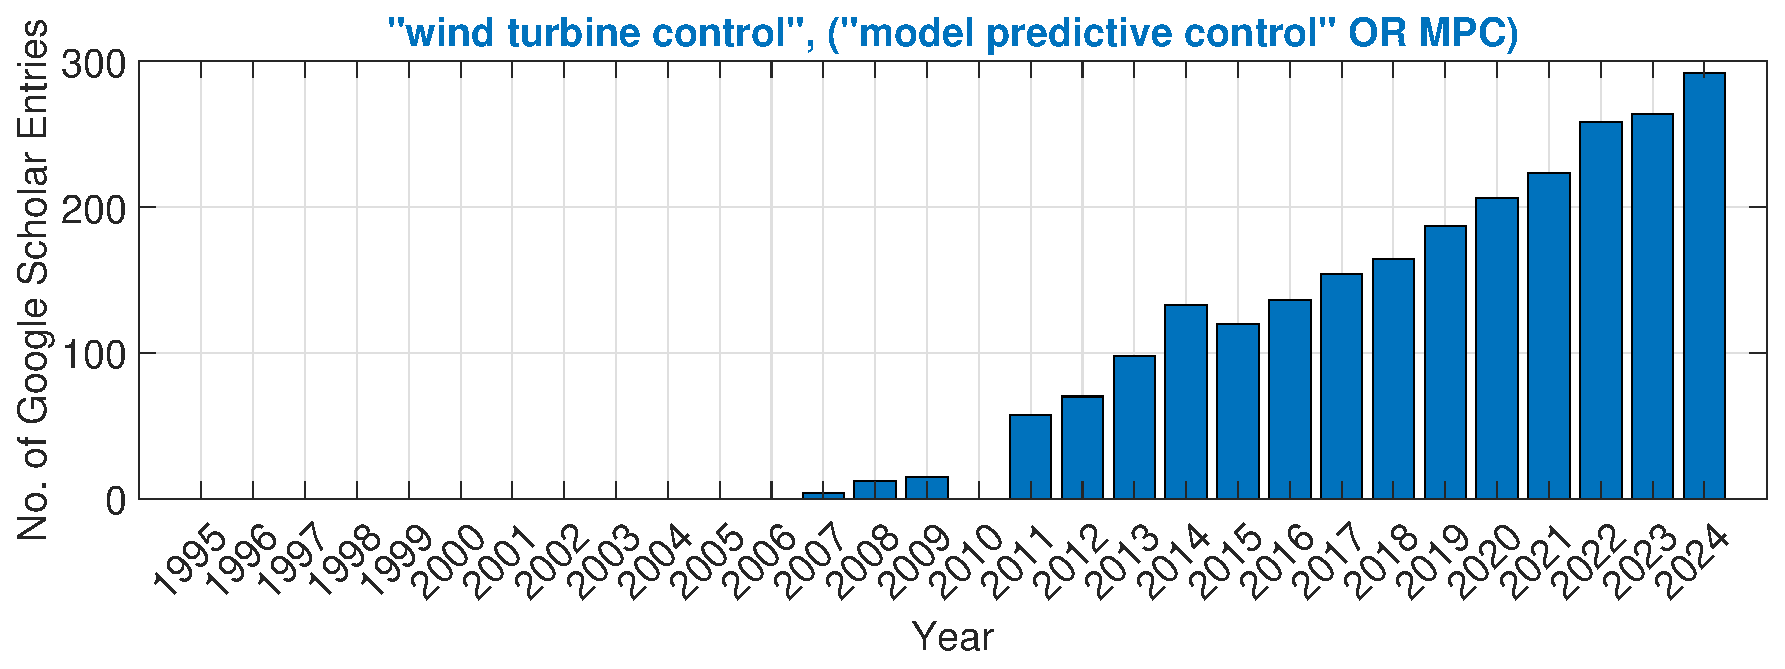
\includegraphics[width=0.85\textwidth]{figures/Figures_ADi/googleWordleWTMPC.eps}} %\hfill
\caption{Number of Google Scholar results by year for the search term ``wind turbine control" and different additional search terms}
\label{fig01:WTstatistics}
\end{figure}

\begin{figure} [h]
 \center
\subfloat[Search terms ``axial induction control" and ``wake redirection control"]{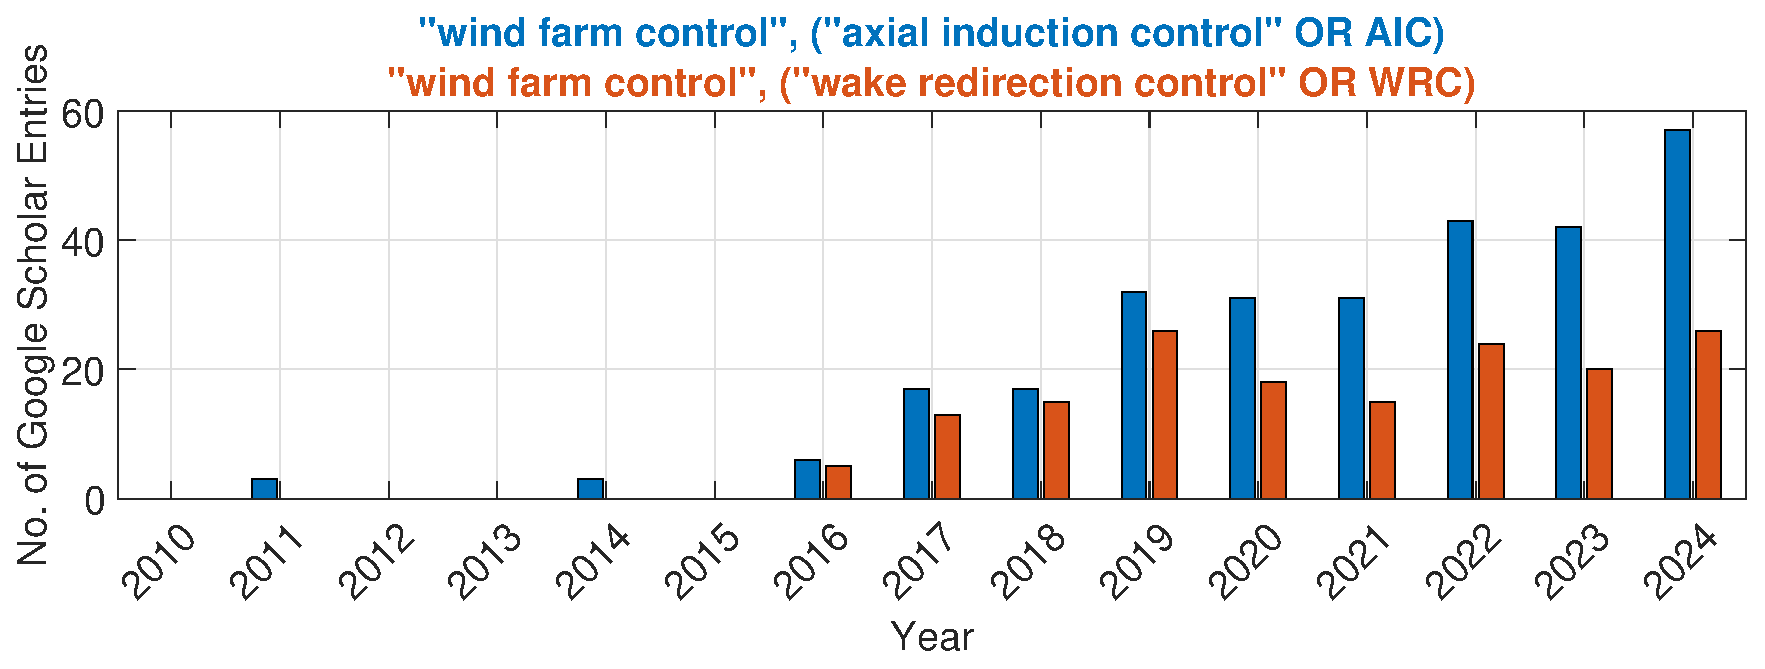
\includegraphics[width=0.85\textwidth]{figures/Figures_ADi/googleWordleWFAICWRC.eps}}\\
\subfloat[Search term ``Koopman"]{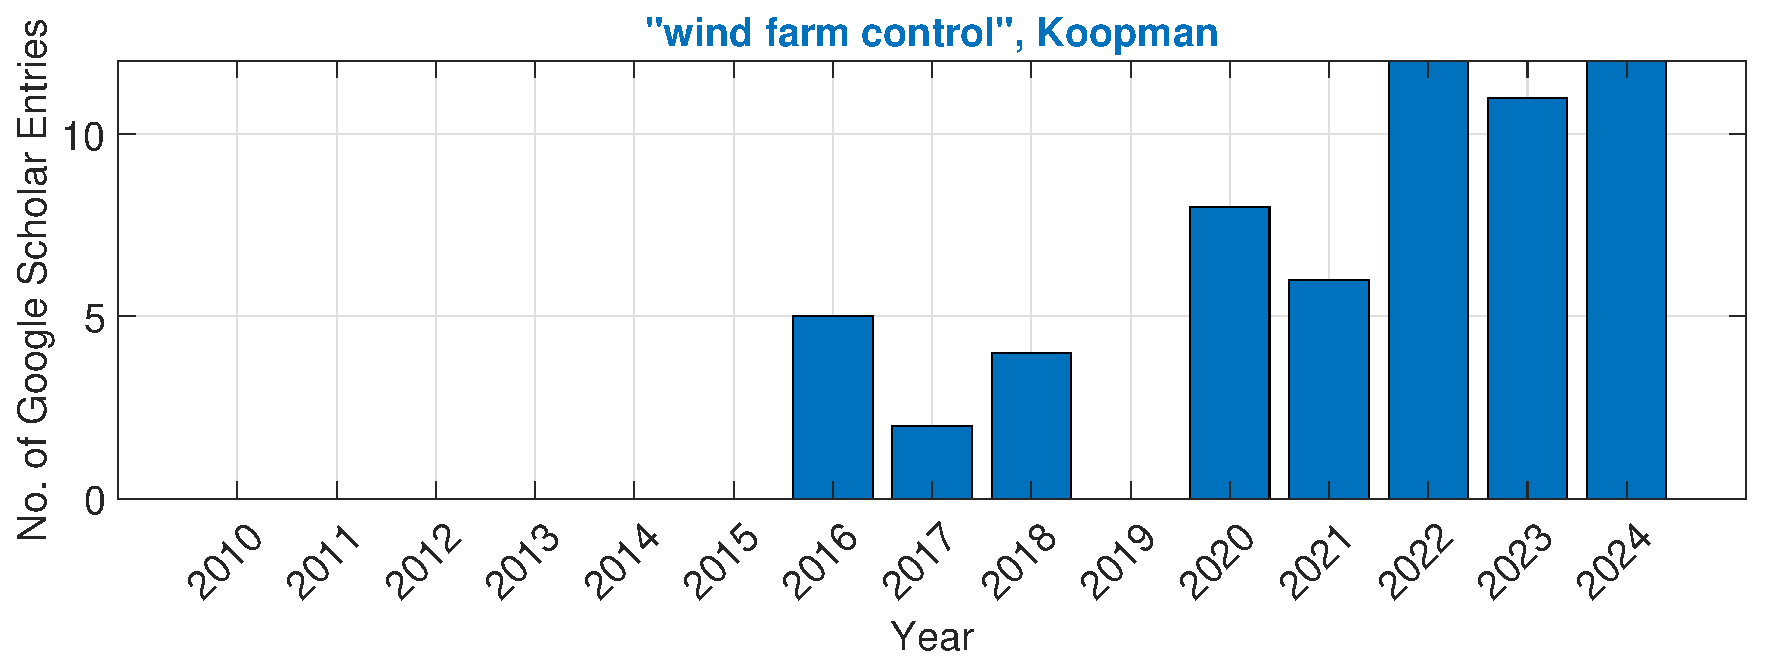
\includegraphics[width=0.85\textwidth]{figures/Figures_ADi/googleWordleWFKoopman.eps}}\hfill
\caption{Number of Google Scholar results by year for the search term ``wind farm control" and different additional search terms }
\label{fig01:WFstatistics}
\end{figure}

Figure~\ref{fig01:WTstatistics}(a) shows a significant increase of number of published studies over the past approximately fifteen years and a continuously high number, exceeding 100 publications each year, after 2021 for both search terms ``load reduction" and ``individual pitch control". Figure~\ref{fig01:WTstatistics}(b) shows a nearly exponential increase in publication number for MPC and wind turbine control, with more than 200 publications found on Google Scholar each year after 2020.  
%
But while there is extensive literature on load reduction of wind turbines, both via IPC, and MPC, relatively few works explicitly examined using quasi-Linear Parameter Varying (qLPV) MPC, so called qLMPC schemes. In \cite{Bianchi2007}, modeling wind turbines as qLPV is described, but not within an MPC, but within an $H_{\infty}$ control approach. In \cite{kumar2010FeedbackLinLQR} a non-linear turbine model is derived and a feedback linearization controller is compared to a Linear Quadratic Regulator (LQR), showing better performance around rated wind speed. The first work to suggest explicitly using the qLMPC introduced in \cite{cisneros2016efficient} for wind turbine control is \cite{mulders2020preventing}, where it is used to derive optimal torque control for tower load reduction as a Single-Input Single-Output (SISO) scheme. This work was followed by a study leveraging a Kalman filter to estimate unmeasurable periodic side-to-side loads in wind turbines, addressing fatigue challenges in tall, slender towers \cite{pamososuryo2022loadestimation}. In \cite{pamososuryo2022individual,pamososuryo2023convex} a convex economic MPC is developed for IPC to actively damp side-to-side tower motion. In \cite{feng2022economic} an economic MPC is used to reduce the load distributed over the turbine tower. Recently, the application of velocity-based qLMPC, an algorithm published in \cite{cisneros2020velocity} for reduction of side-to-side tower motion was investigated in \cite{fonseca2024windTurbineSideSide}. In parallel, IPC has been applied in various studies to enable blade root moment reduction: Promising simulation results exist with different control algorithms, e.g., Proportional-Integral-Derivative (PID) \cite{hoffmann2018load}, Linear Quadratic Gaussian (LQG) \cite{selvam2009feedback}, and MPC schemes \cite{petrovic2021mpc}. Field tests confirm the potential of IPC, see \cite{ossmann2021field} and \cite{bossanyi2012advanced}. Recently, TEFs for wind turbines have been suggested for blade root load reductions in \cite{zhang2015parameter} and \cite{bergami2017highfidelity}. As TEF add an additional degree of freedom to the wind turbines' actuation, there are also studies combining the two methods: In \cite{wilson2009combined}, the standard deviation of blade root flapwise bending moments is reduced up to 32\% for two wind test cases with turbulence class A, at 16\,m/s and 20\,m/s mean wind speed. Turbulence class A at 18\,m/s mean wind speed is used in \cite{henriksen2013model} to investigate the trade-off between load reduction and actuator activity. In \cite{he2018combined}, the blade root flapwise moments and blade tip out-of-plane deflection are both reduced by over 50\%, while also decreasing tower moments for a wind test case of turbulence class B at 20\,m/s. In Chapter~\ref{sec:WindTurbineqLPVModels} of this thesis the design of two qLPV models, one modelling the tower and rotor dynamics as proposed in the previously cited studies and one additionally including blade and generator dynamics as suggested in \cite{Bianchi2007} is presented. In Chapter~\ref{sec:Application to Wind Turbine Control4} the implementation of a velocity-based qLMPC controller is discussed, with a focus on power reference tracking and fore-aft tower motion reduction. This is followed by the design and evaluation of an IPC controller and a combined IPC–TEFC control strategy, which are directly compared to the qLMPC scheme across multiple performance criteria.

Similarly to wind turbine control, Figure~\ref{fig01:WFstatistics}\,(a) shows that for the last ten years wind farm control is a widely studied subject, but that the number of studies leveraging Koopman theory is more limited, see Figure~\ref{fig01:WFstatistics}\,(b). The survey paper \cite{houck2022review} categorizes wake management into AIC, WRC, a combination of WRC-AIC, and active wake control. Currently, WRC, which uses yaw to redirect wakes, is the most frequently investigated technique and likely to achieve broader industrial application. However, applying WRC to real wind turbines will require combining it with thrust control via power control for below-rated wind speeds and pitch control for above-rated wind speeds.

Of the 8 papers mentioned in \cite{houck2022review} to use combined WRC-AIC, \cite{jimenez2010application} investigates the wake centerline deflection and spread in simulations and \cite{castillo2020wind} in wind tunnel tests. In \cite{bossanyi2018combining} an increase in production and decreased loads, both in the lower one-digit percentage range, is demonstrated in simulations. A lower two-digit percentage increase in power is reported in \cite{cossu2020wake}, based similarly on simulations. In \cite{fleming2016computational} it is concluded that combined WRC-AIC is the control technique resulting in the lowest grid reference tracking error. In the three papers, \cite{park2013wind}, \cite{park2015cooperative}, and \cite{en10070852}, the authors use different, purely data-driven techniques to optimize a combination of induction and yaw control. The advantage of combined WRC-AIC is summarized in \cite{houck2022review} by noting that lowering the thrust of the upstream, misaligned turbine may provide the optimal balance of power increase and load reduction, if wake steering is insufficient to steer a wake completely away from a downstream turbine. But it is mentioned that combined WRC-AIC still requires prior optimizations or real-time computing to implement in the field. However, with a data-driven technique like Koopman MPC a real-time controller can be implemented for wind farms. 

The idea of using the Koopman matrix, a linear approximation of the Koopman operator, to model wind flow and wakes in a wind farm was first suggested in \cite{annoni2016wind} and extended to farm control via axial induction control in \cite{annoni2016sparsity}. The potential of Dynamic Mode Decomposition (DMD) for wake models was also pointed out in \cite{proctor2016including} which provides a comparison between DMD and the proper orthogonal decomposition for fluid dynamics modelling. In \cite{munters2017optimal} a MPC is set up with the wind farm dynamics modelled as Large Eddy Simulation (LES) and hence based on Navier-Stokes Equation (NSE) and in \cite{munters2018data} the idea of using Koopman to model LES is discussed. In \cite{debnath2017towards} the structure of a wake, simulated via LES, is analyzed. Based on their previous work, it is discussed \cite{annoni2018sparse} how lidar sensors are to be placed in wind farms to extract a maximum amount of information. In \cite{ali2020data} the varying flow velocities over the blade span are modelled with a linear model derived via an Extended DMD (EDMD), taking the forces acting on the rotor excited by the control inputs into account. \cite{chen2020data} discusses using DMD to model the wake flow dynamics. A proof-of-concept for Koopman matrices derived via  Extended Input-Output DMD (EIODMD), with the resulting linear state-space models used as basis for MPC, is given in \cite{Cassamo.2020}, which investigates AIC, and in \cite{cassamo2021model} for WRC. In Chapter~\ref{sec:ApplicationtoWindFarmControl} of this thesis the application of Koopman MPC to AIC as well as a combination of AIC and WRC is discussed. 

\section{Main Contributions}
This section outlines the primary contributions of this thesis in the field of wind turbine and wind farm control. The research focuses on the integration of novel physics-based and data-driven MPC techniques to optimize wind turbine and wind farm performance. In all contributions, care was taken to make the algorithms real-time capable, with convergence rates considerably below the 10\,ms sampling rate of wind turbine controller, and to only use input signals that can realistically be expected to be available during the operation of a real wind turbine. Although the applicability of these algorithms remains at the proof-of-concept stage, they could be applied to wind turbine control with relatively little modification, assuming the necessary sensors and actuators are available. 

The first contribution of this thesis is the development of a real-time capable, velocity-based qLMPC for wind turbine control across the entire operating range. Leveraging Lagrange's equations, a first-principles model incorporating the physics, mechanics, and aerodynamics of the wind turbine was formulated. This model was then utilized in an MPC framework, reformulated as a Quadratic Programming (QP) problem to achieve real-time convergence within millisecond timescales. This work was published in \cite{dittmer2021velocity}.
%
Furthermore, the development and rigorous verification of an active aerodynamic load control system integrating IPC with TEF control is presented. While previous studies had suggested the potential of combining IPC and TEF for wind turbine control, our study, published in \cite{dittmer2024combined}, was the first to rigorously demonstrate the effectiveness of this approach across a wide range of wind speeds. The research evaluated the FAST turbine model extended  with TEFs, using a training dataset and two independent verification datasets, to ensure a comprehensive performance assessment. The results confirmed a significant reduction in blade root out-of-plane moments and tower base loads.

The second contribution is the development of an adaptive Koopman MPC framework for wind farm control, marking the first time this efficient update mechanism has been applied in wind farm control simulation. Inspired by the Navier-Stokes equations governing turbine interaction, this approach leverages Koopman lifting functions to construct a Koopman matrix for predicting wake interactions and effective wind speed. Computational efficiency is achieved by updating the Koopman matrix only when discrepancies between past predicted and actual wind data are detected. This work builds upon prior research on qLMPC for wind farm control, enhancing its applicability by highlighting its potential to adapt to sudden changes in operation. The findings were published in \cite{dittmer2022data}, extending our earlier work on non-adaptive MPC \cite{sharan2022Koopman}.

Additionally, a data-driven Koopman MPC approach for combined thrust and yaw control in wind farms is demonstrated. Combining thrust and yaw control was motivated by the fact that, due to the slowness of yaw movements, practical implementations of WRC must be combined with pitch and torque control for dynamic load management and efficient power regulation. This combination is driven by the superior power yields achievable with WRC compared to AIC. By incorporating WRC-AIC into the previous AIC framework, this approach achieved a roughly 10\% increase in power output under steady-state conditions and enabled the system to follow grid power references with higher power demands. This data-driven approach directly estimates farm power using a linear system based on the Koopman matrix, eliminating the need for detailed wake modeling. The Koopman MPC framework, presented in \cite{dittmer2023koopman}, demonstrates promising results in achieving reference tracking at reduced actuator activity.

The effectiveness of the proposed MPC controllers is validated through comparative analyses against non-predictive schemes and baseline MPC approaches. Results indicate improvements in power tracking, load reduction, and control quality. Additionally, the wind farm Koopman MPC demonstrates performance with reduced measurement requirements, offering practical advantages over solutions presented in previous studies.

\section{Thesis Structure}
This thesis is organized as follows: Chapter \ref{sec:Background} provides a comprehensive review of the physics of wind, wind turbine and wind farm dynamics, and their control. The fundamental ideas of qLPV models and MPC are presented. The chapter also introduces the Koopman operator and DMD.

Chapter~\ref{sec:WindTurbineqLPVModels} focuses on the development of a qLPV wind turbine model. Two models are derived: one modeling the rotor speed and tower movements only, and one, using Lagrange's equations, modeling additionally blade movements and generator speed. The quality of the two qLPV models is verified across the entire turbine operating range in both frequency and time domains using the software FAST.

Chapter~\ref{sec:Application to Wind Turbine Control4} presents the work on wind turbine control, encompassing both the velocity-based qLMPC framework and the active aerodynamic load control system integrating IPC with TEF control. The qLMPC framework is discussed in terms of its reformulation as a  QP problem for real-time implementation. Its performance is evaluated for power tracking and load reduction, with comparative analyses against baseline control methods. The chapter also discusses the effectiveness for reducing blade root and tower loads over a wide range of wind speeds with the IPC-TEF approach.   

Chapter~\ref{sec:ApplicationtoWindFarmControl} describes Koopman MPC for wind farm control: an adaptive Koopman MPC using thrust control and a Koopman MPC for combined thrust and yaw control. The software WFSim and enhancements necessary to evaluate the presented algorithms are discussed. The adaptive Koopman MPC leverages efficient update mechanisms to deal with abrupt changes, while the combined thrust and yaw approach integrates WRC with AIC to increase power yield. The chapter evaluates the proposed methods for power output improvement, grid reference tracking, and actuator activity reduction.

Chapter~\ref{Conclusions} summarizes the main contributions and findings of the thesis 
and discusses the practical implications of the proposed control strategies. It provides 
a discussion of existing challenges, concretely relating to sensor 
integration, actuator degradation, and validation in higher-fidelity simulation 
environments. Finally, it outlines directions for future research, including the 
extension to more realistic wind conditions and the use of Neural Network~(NN) based 
lifting functions as an alternative to physically motivated observables.


